\documentclass[abstract=on,9pt,twocolumn]{scrartcl}

\usepackage{ucs}
\usepackage[utf8x]{inputenc}
\usepackage[T1]{fontenc}
\usepackage[english]{babel}
\usepackage{datetime}
%\usepackage{multicol}

\usepackage[paper=a4paper,top=2cm,left=1.5cm,right=1.5cm,bottom=2cm,foot=1cm]{geometry}

\usepackage{relsize}%	relative font sizes

\usepackage[retainorgcmds]{IEEEtrantools}%	IEEEeqnarray
\setlength{\IEEEnormaljot}{4\IEEEnormaljot}

\usepackage{graphicx}
\usepackage{epstopdf}
\usepackage{indentfirst}
\usepackage{hyperref}
% \usepackage{cleveref}
\usepackage[noabbrev]{cleveref}
\usepackage{listings}
\usepackage{color}
\usepackage{subfig}

%%%%%%%%%%%%%%%%
%  title page  %
%%%%%%%%%%%%%%%%
%\titlehead{University of Minho \hfill Master's Degree in Informatics Engineering\\Department of Informatics \hfill Parallel and Distributed Computing}

\title{GMetis - Xeon Phi}

\author{
    \\David Pereira\\
     	\texttt{\smaller pg22821@alunos.uminho.pt}
\\~\\~
\and\\Rui Brito\\
	\texttt{\smaller pg22781@alunos.uminho.pt}
}

\date{Austin, \docdate}

%%%%%%%%%%%
%  Hacks  %
%%%%%%%%%%%

%	Paragraph (title) with linebreak
\newcommand{\paragraphh}[1]{\paragraph{#1\hfill}\hfill

}

%	Add "Appendix" to the appendices titles, but not to the references
\usepackage{ifthen}
\newcommand*{\appendixmore}{%
  \renewcommand*{\othersectionlevelsformat}[1]{%
    \ifthenelse{\equal{##1}{section}}{\appendixname~}{}%
    \csname the##1\endcsname\autodot\enskip}
  \renewcommand*{\sectionmarkformat}{%
    \appendixname~\thesection\autodot\enskip}
}

\newdateformat{mmmyyyydate}{\monthname[\THEMONTH] \THEYEAR}
\newcommand{\docdate}{\mmmyyyydate\today}


%-----------------------------------------------------------------------------
% Cenas a falar
%-----------------------------------------------------------------------------

% USA W -> o maior grafo possivel de correr no MIC devido a limitações
% de memória

% Correr o Metis num core do MIC? Em vez de correr no Host?



%-----------------------------------------------------------------------------
% Begin Document
%-----------------------------------------------------------------------------

\begin{document}
\maketitle	


%-----------------------------------------------------------------------------
% Abstract
%-----------------------------------------------------------------------------

\begin{abstract}

\end{abstract}


%-----------------------------------------------------------------------------
% Introduction
%-----------------------------------------------------------------------------

\section{Introduction}



%-----------------------------------------------------------------------------
% Metis Algorithm Description
%-----------------------------------------------------------------------------

\begin{itemize}
  \item GMetis is a graph partitioning application which uses the Galois
    framework
  \item Consists of three major phases
    \begin{itemize}
      \item Coarsening
      \begin{itemize}
        \item Find matching nodes
        \item Create Coarse Edges
      \end{itemize}
      \item Initial Partitioning (Clustering)
      \item Refinement
    \end{itemize}
\end{itemize}

\begin{itemize}
  \item Given a graph $G_0 = (V_0,E_0)$:
  \begin{itemize}    
    \item Coarsening
    \begin{itemize}
      \item $G_0$ is transformed into a sequence of smaller graphs $G_1,G_2,\cdots,G_m$ such that $|V_0|>|V_1|>|V_2|>\cdots>|V_m|$
    \end{itemize}
    \item Partitioning 
    \begin{itemize}
      \item A 2-way partition $P_m$ of the graph $G_m = (V_m,E_m)$ is computed that partitions $V_m$ into two parts, each containing half the vertices of $G_0$
    \end{itemize}
    \item Refinement
    \begin{itemize}
      \item The partition $P_m$ of $G_m$ is projected back to $G_0$ by going through intermediate partitions $P_{m-1}, P_{m-2},\cdots,P_1,P_0 $
    \end{itemize}
  \end{itemize}
\end{itemize}

%\begin{columns}[c]
  %\column{.45\textwidth}{}
  %\scriptsize
  %\begin{center}
    %\begin{figure}[htbp]
      %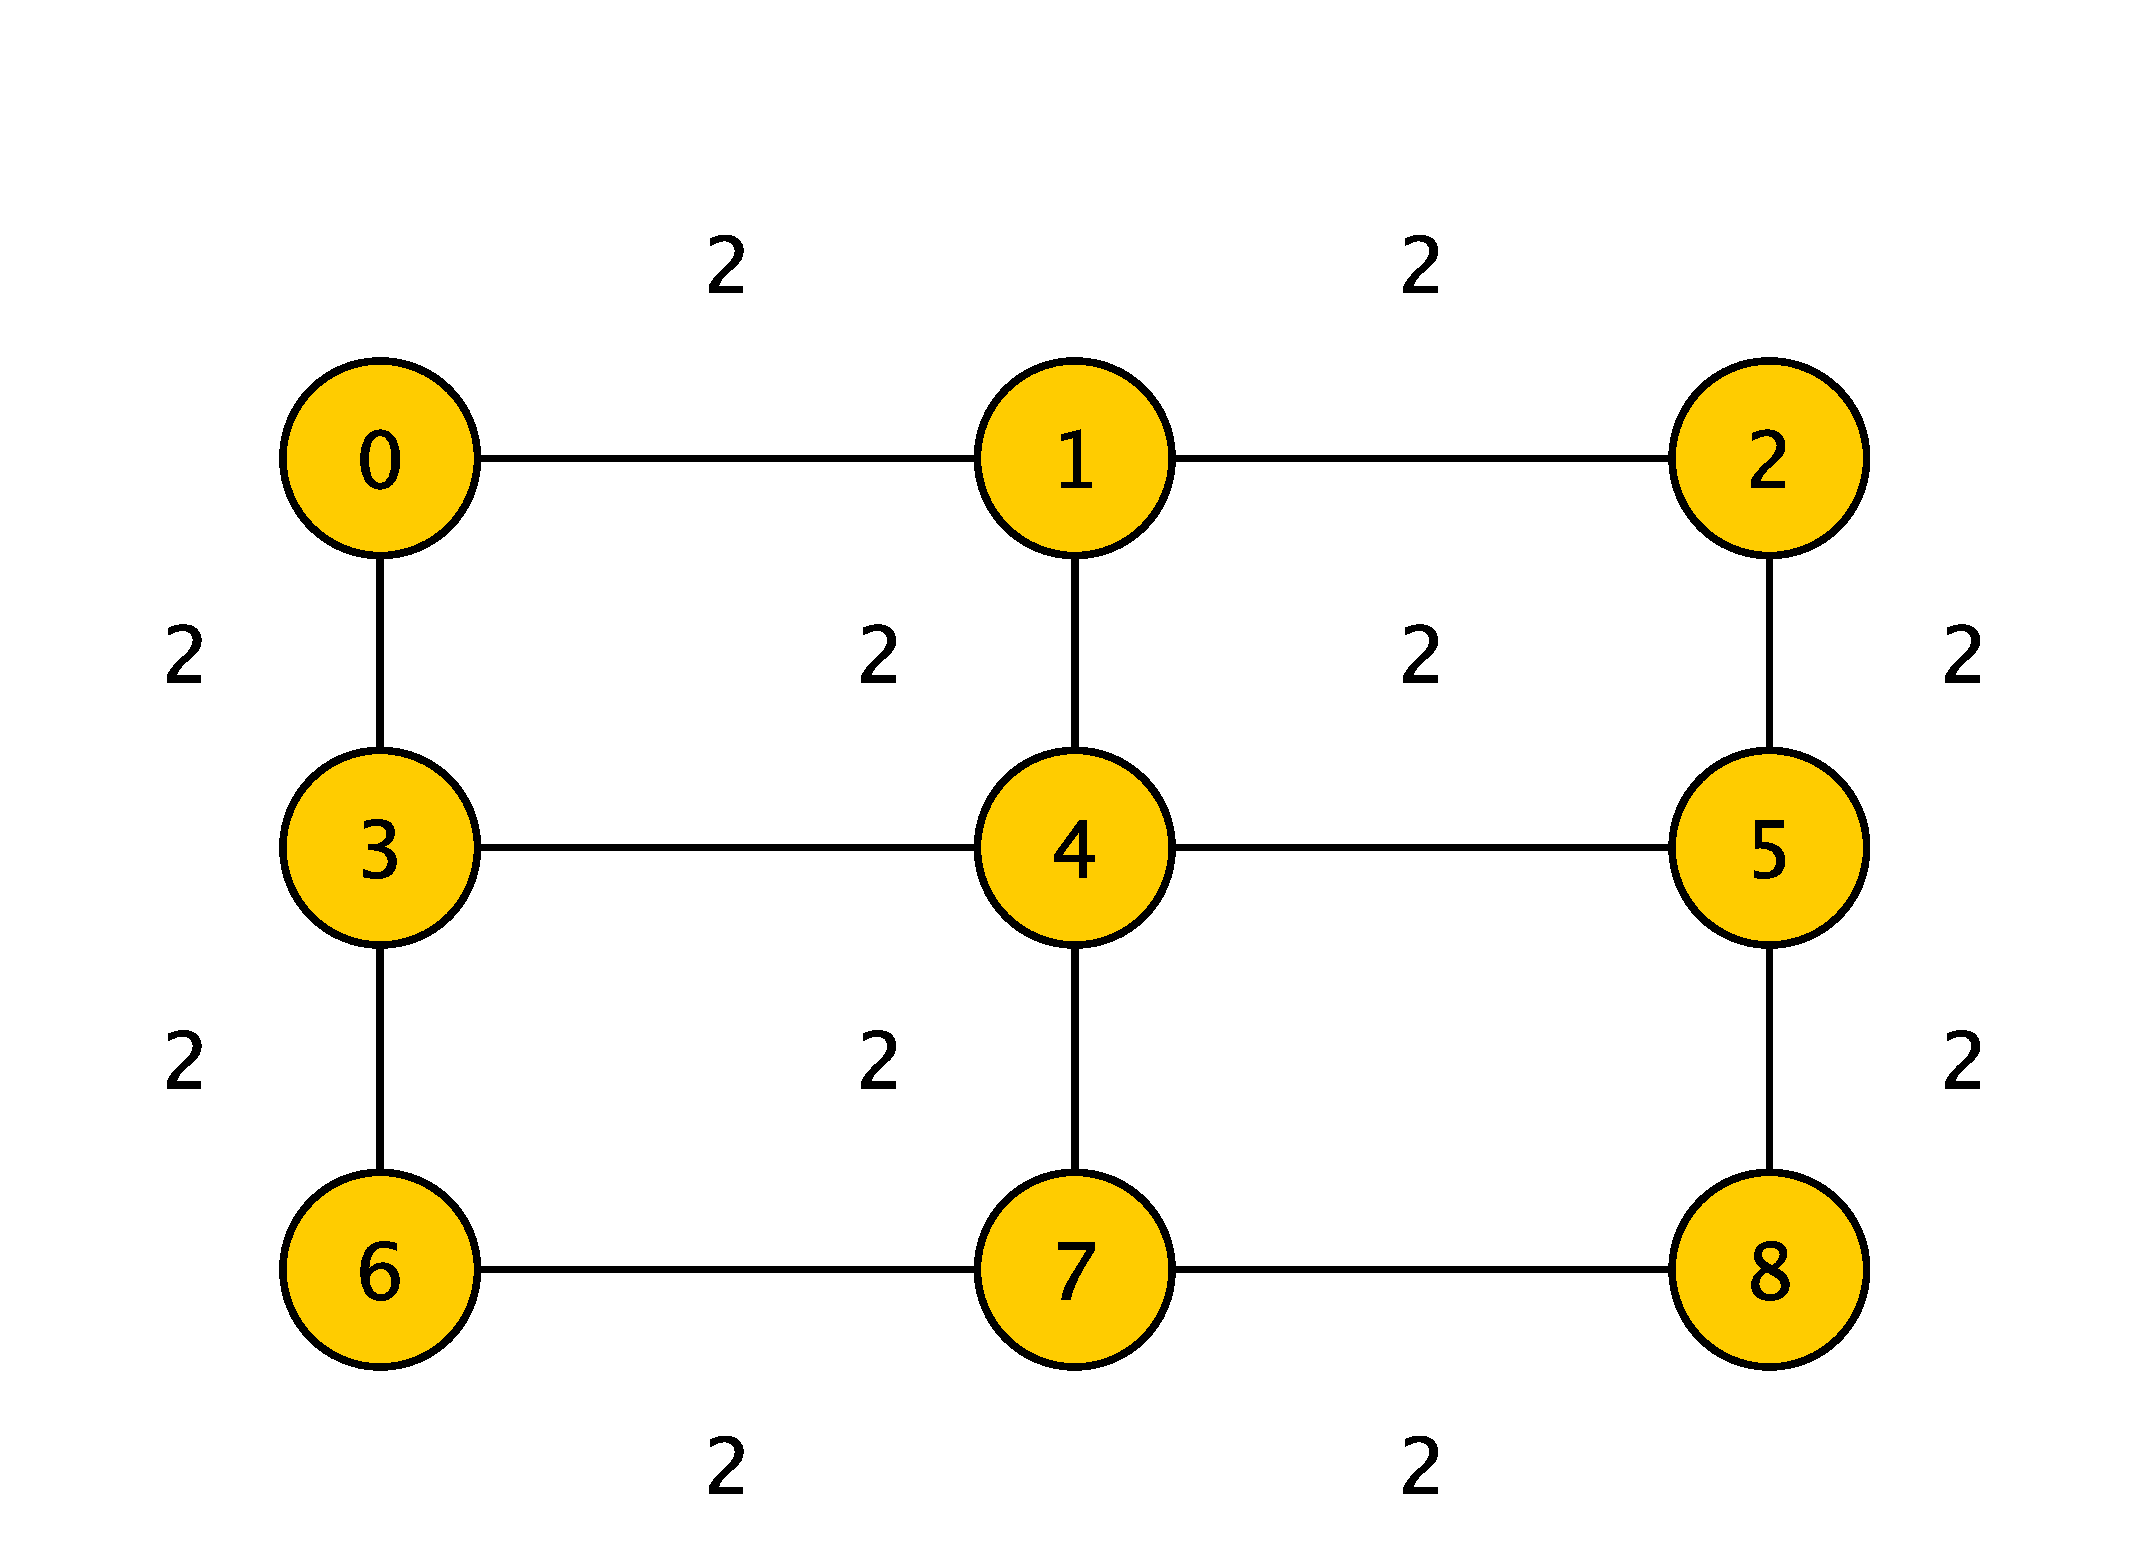
\includegraphics[scale=.15]{img/coarsening.eps}
    %\end{figure}
  %\end{center}

  %\column{.05\textwidth}{} 
  %\begin{center}
    %$\longrightarrow$  
  %\end{center}    
  
  %\column{.45\textwidth}{} 
  %\begin{center}
    %\begin{figure}[htbp]
      %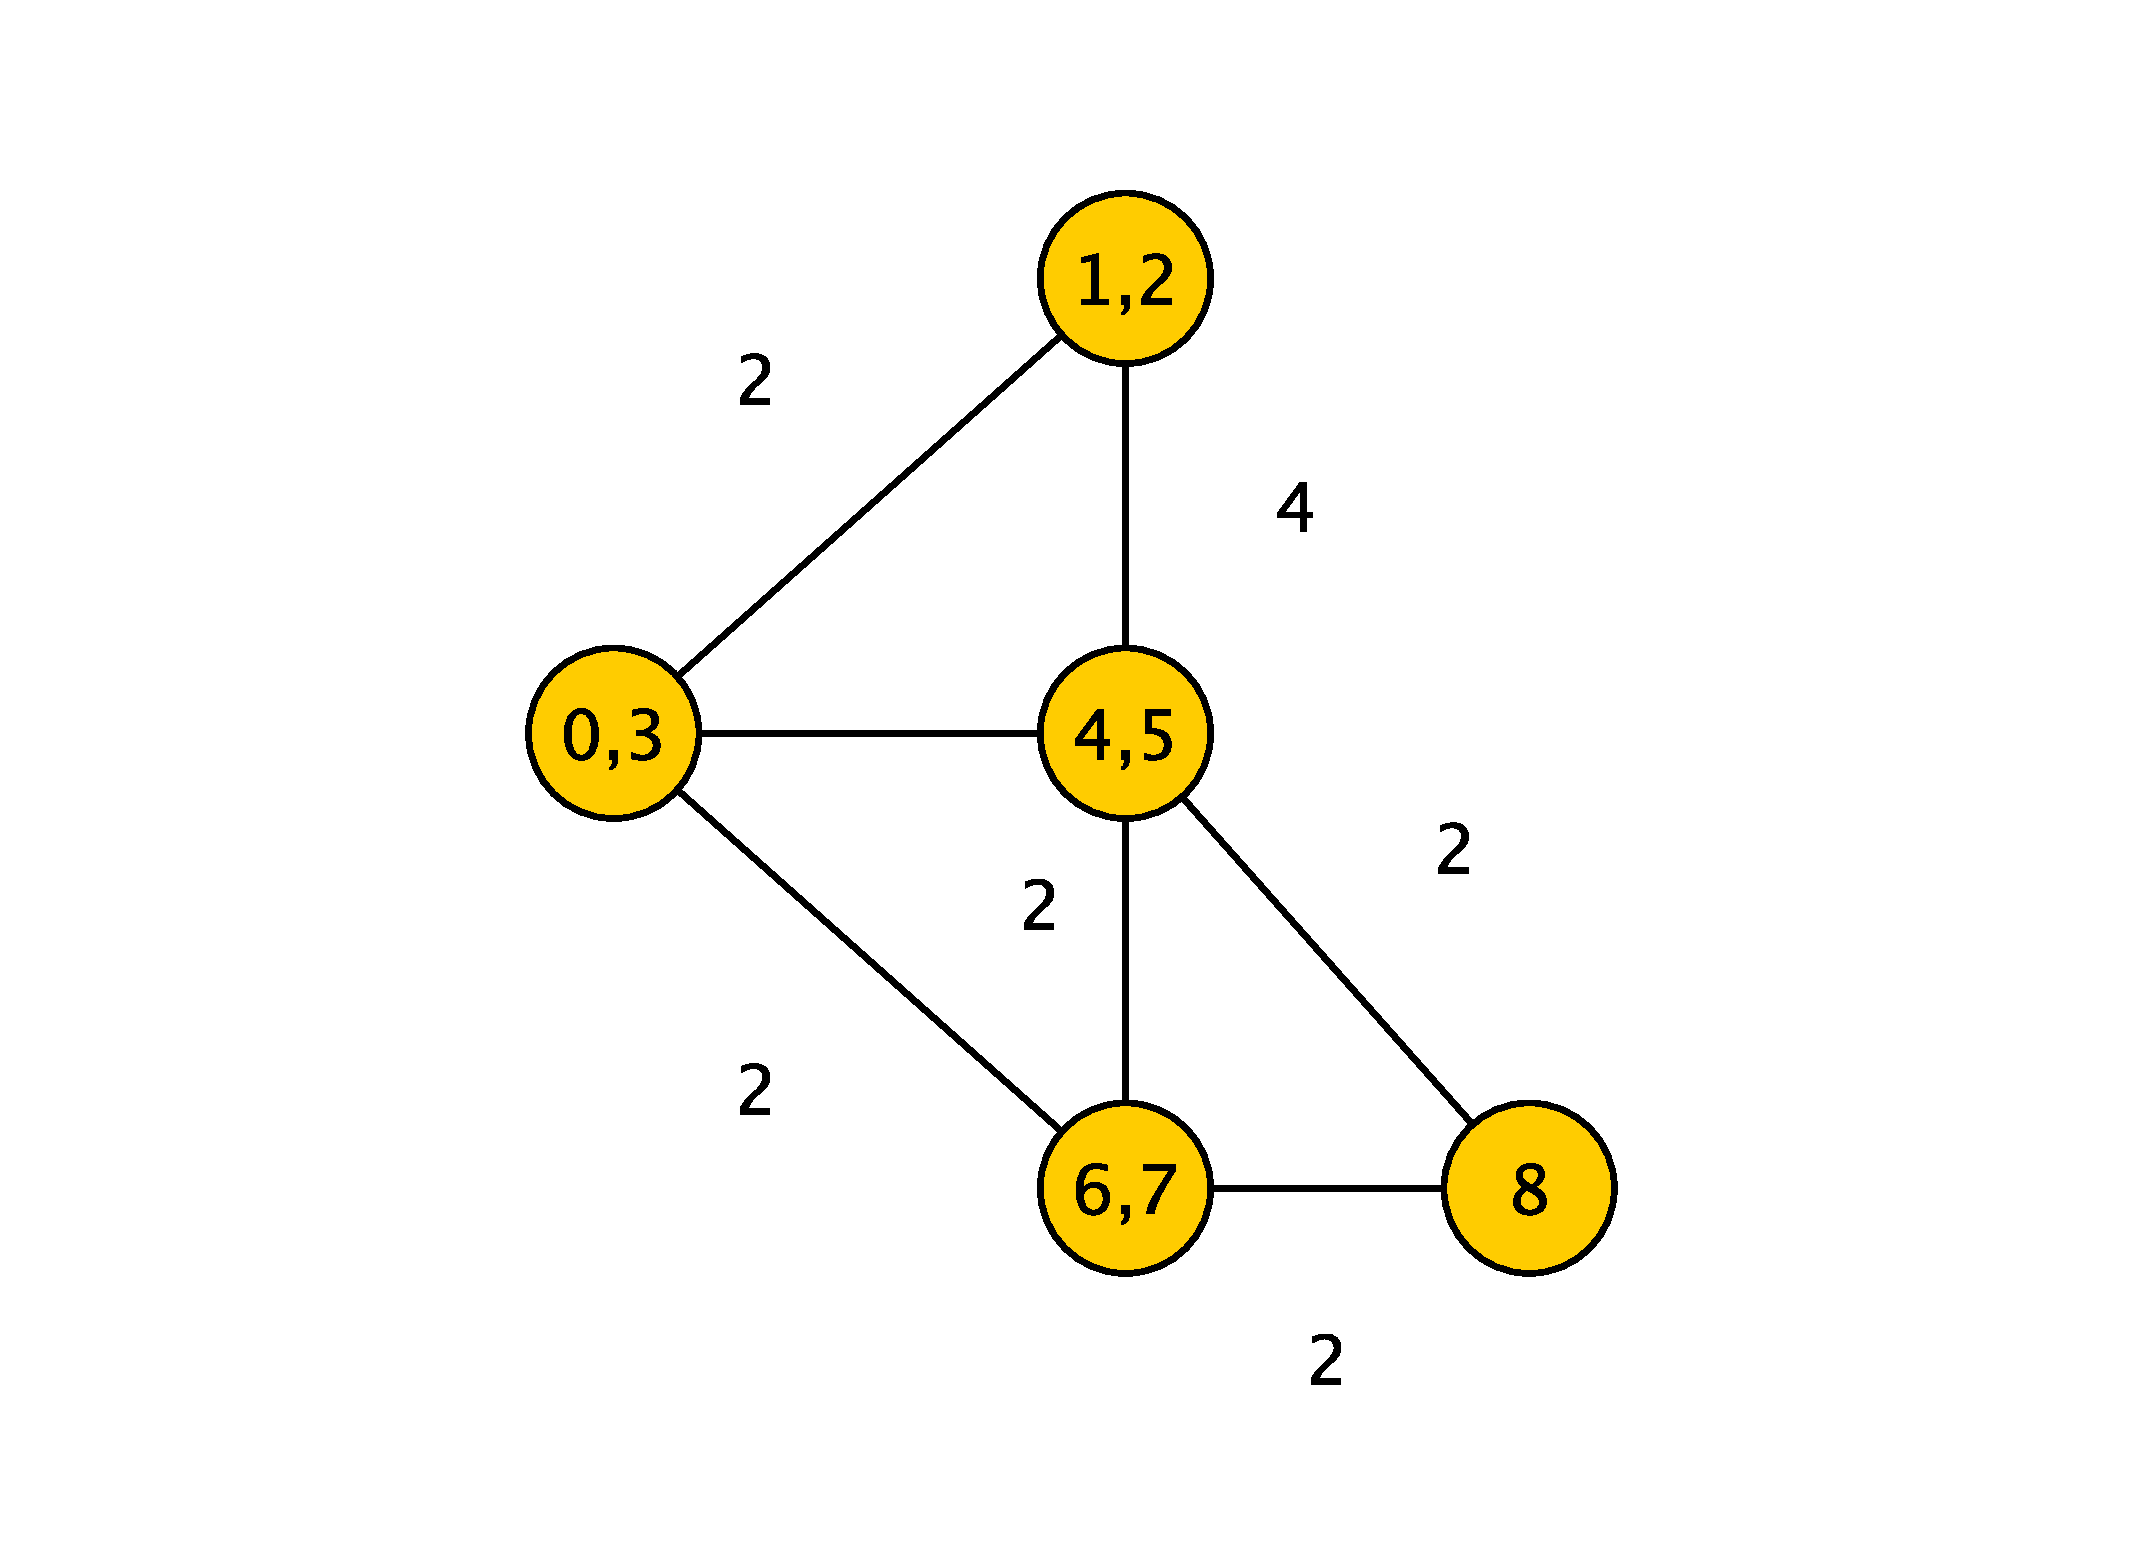
\includegraphics[scale=.15]{img/coarsening2.eps}
    %\end{figure}
  %\end{center}

%\end{columns}


%\begin{columns}[c]
  %\column{.45\textwidth}{}
  %\scriptsize
  %\begin{center}
    %\begin{figure}[htbp]
      %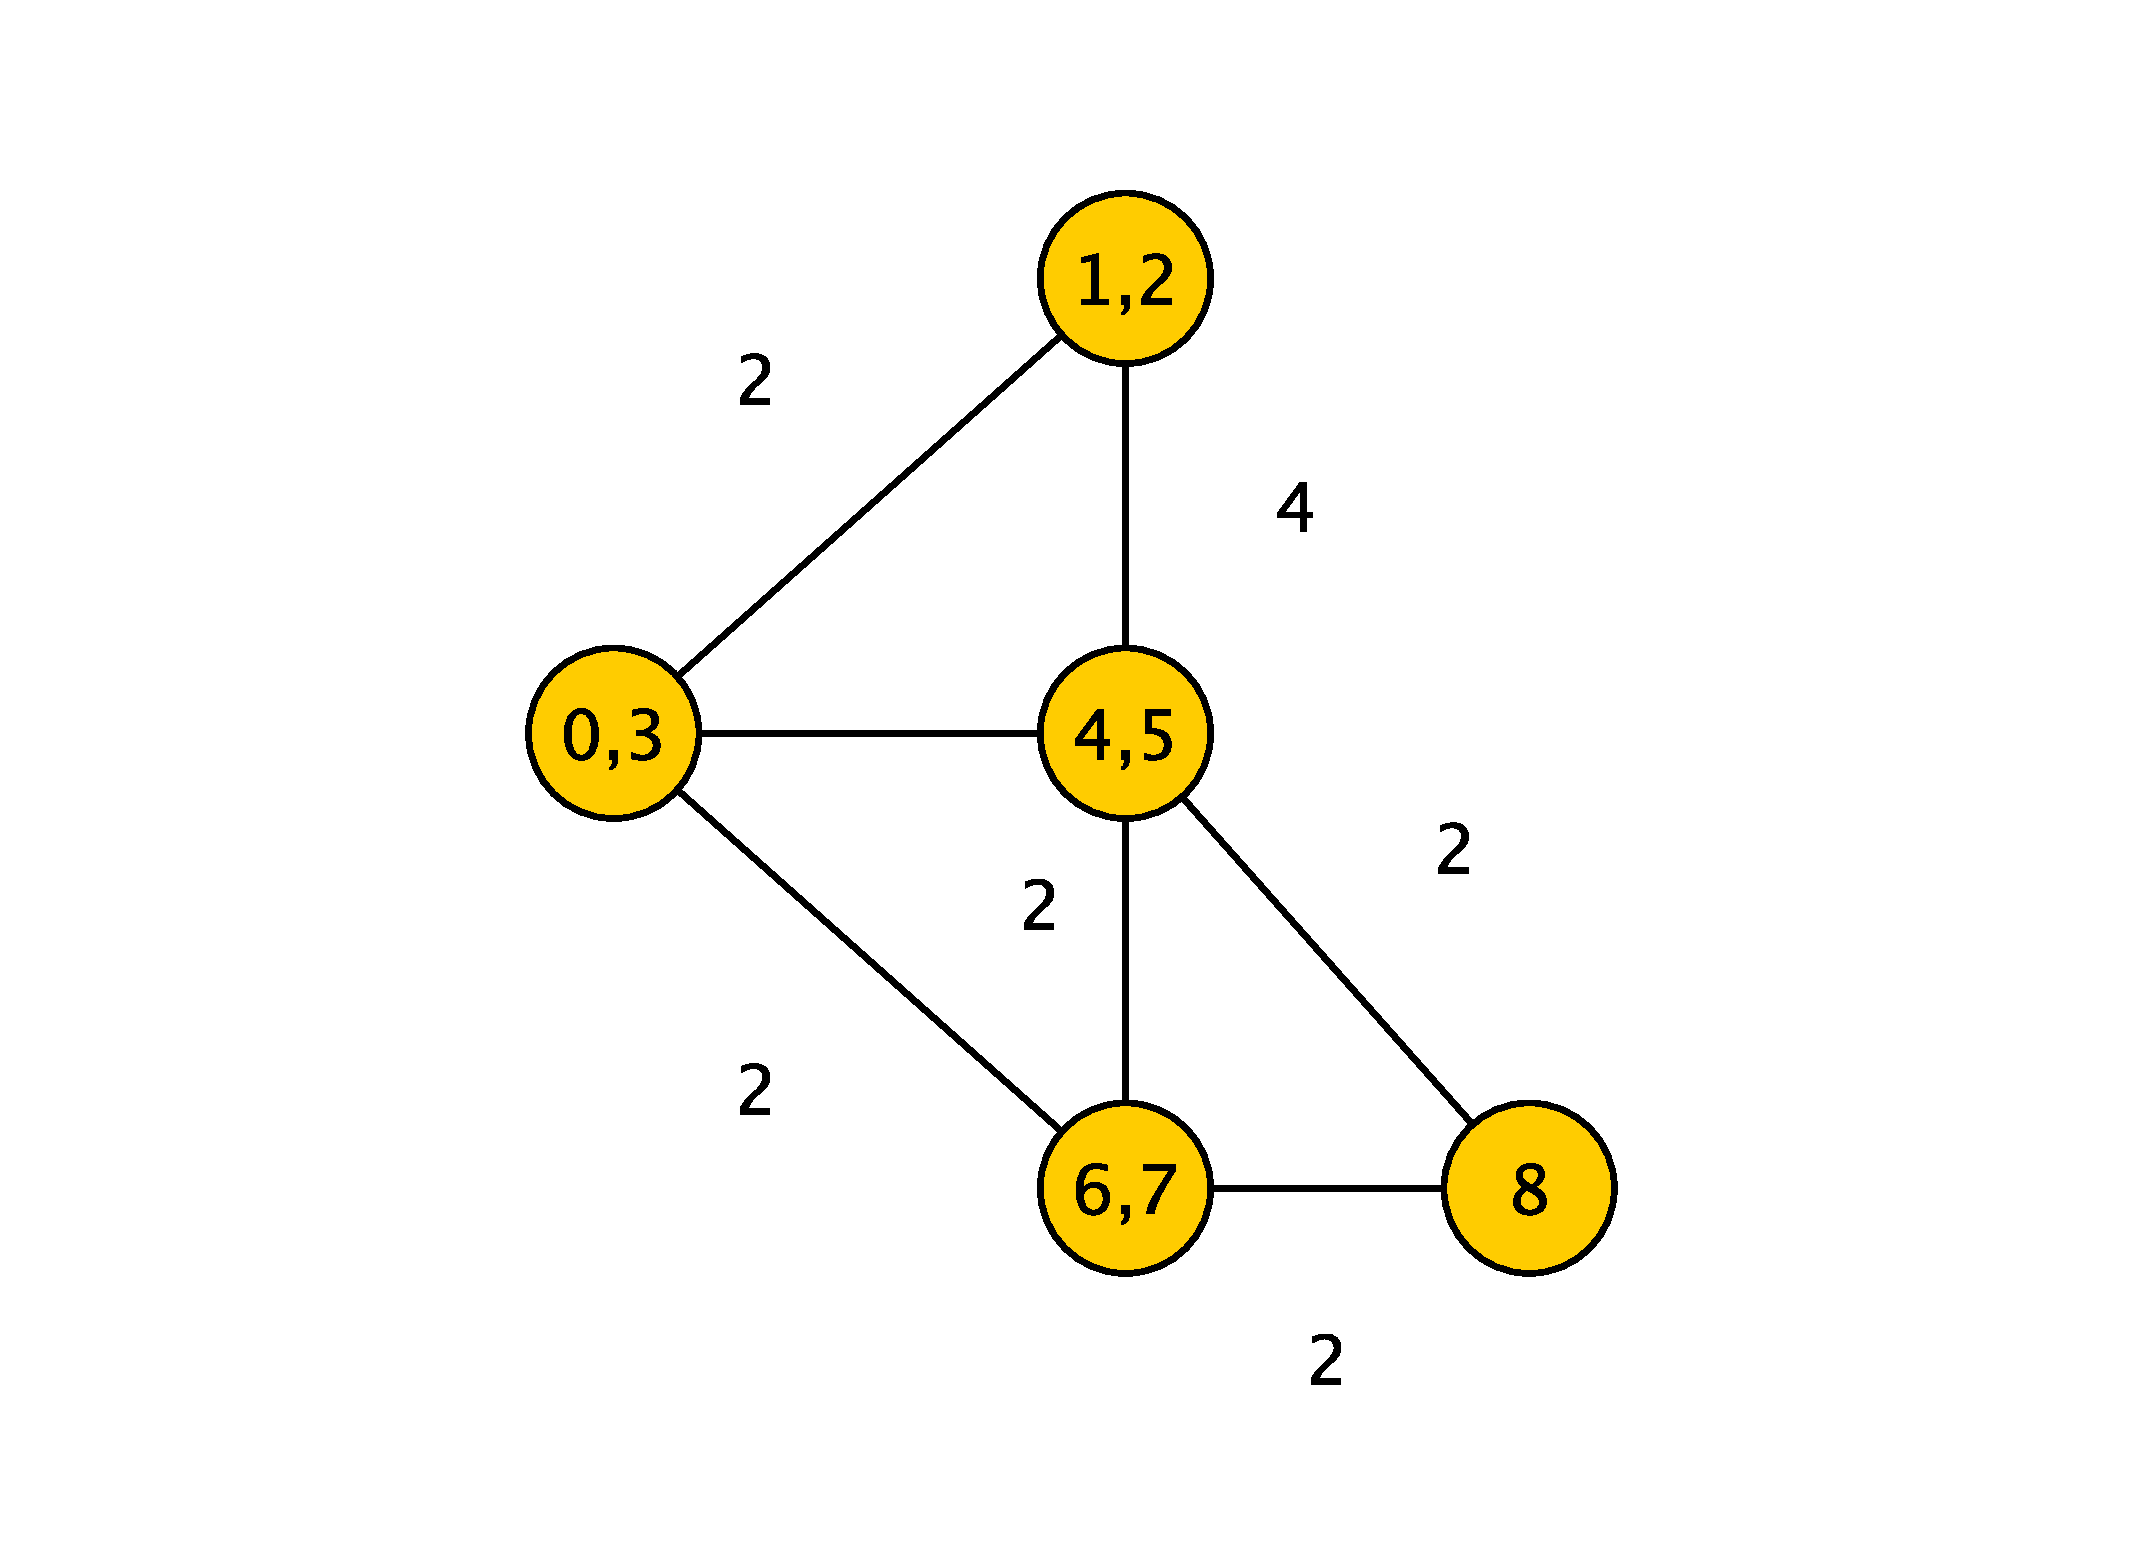
\includegraphics[scale=.15]{img/coarsening2.eps}
    %\end{figure}
  %\end{center}

  %\column{.05\textwidth}{} 
  %\begin{center}
    %$\longrightarrow$  
  %\end{center}    
  
  %\column{.45\textwidth}{} 
  %\begin{center}
    %\begin{figure}[htbp]
      %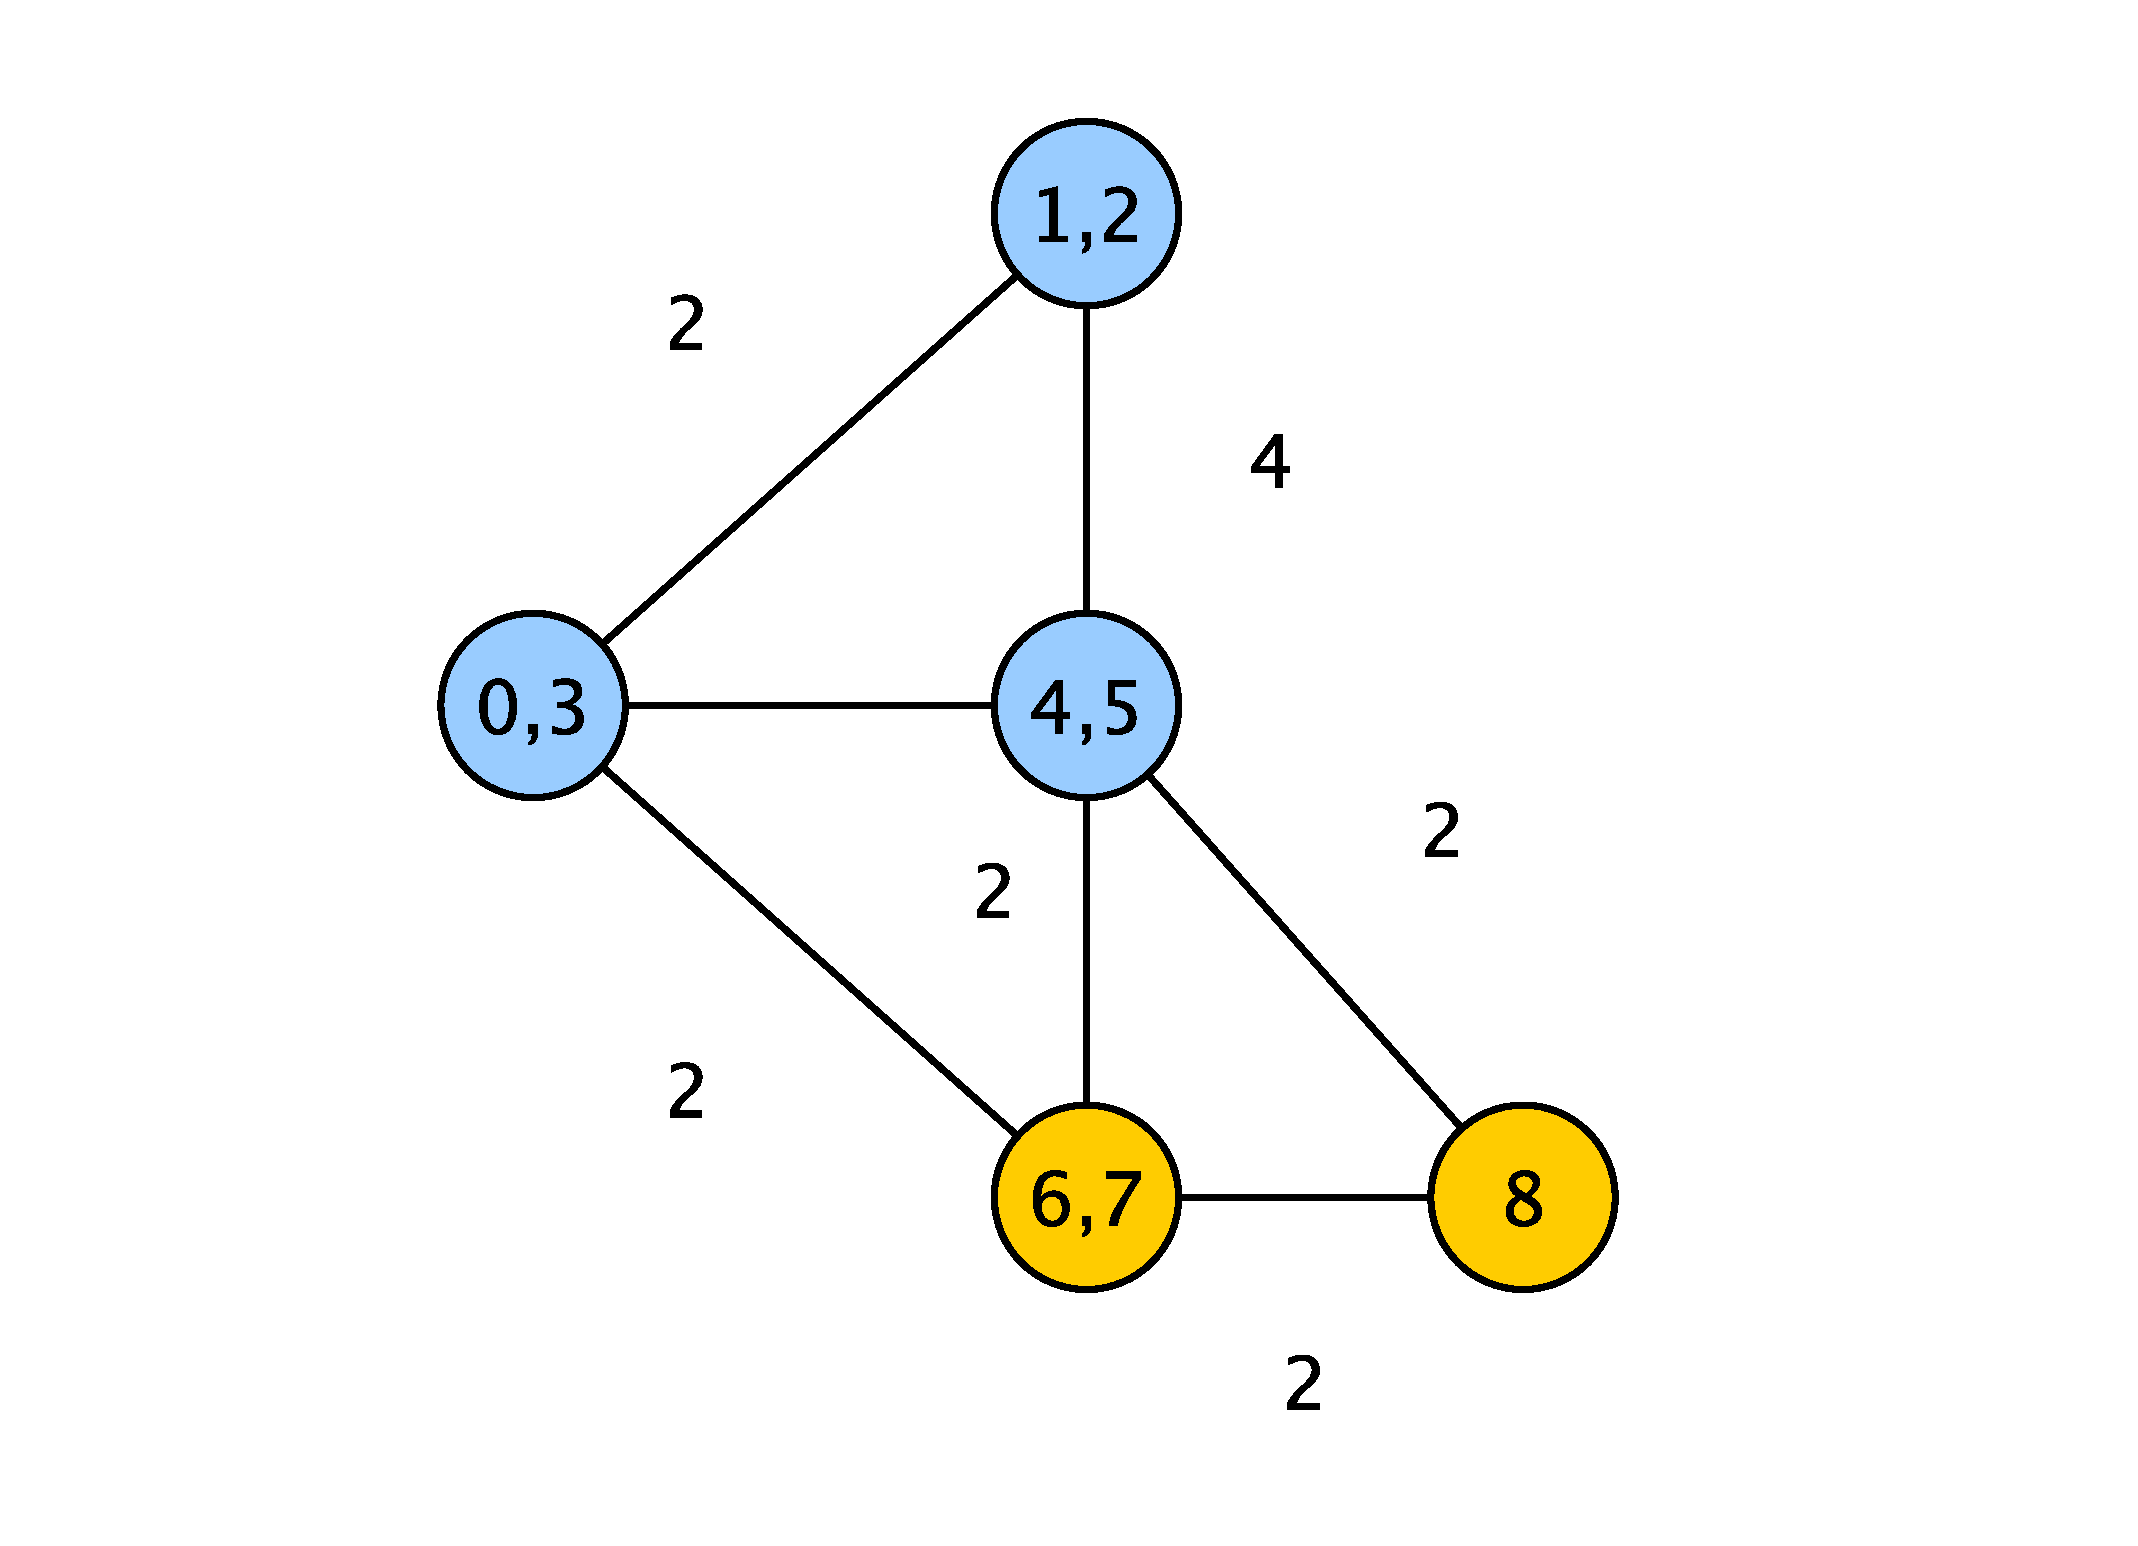
\includegraphics[scale=.15]{img/partition.eps}
    %\end{figure}
  %\end{center}

%\end{columns}


%\begin{columns}[c]
  %\column{.45\textwidth}{}
  %\scriptsize
  %\begin{center}
    %\begin{figure}[htbp]
      %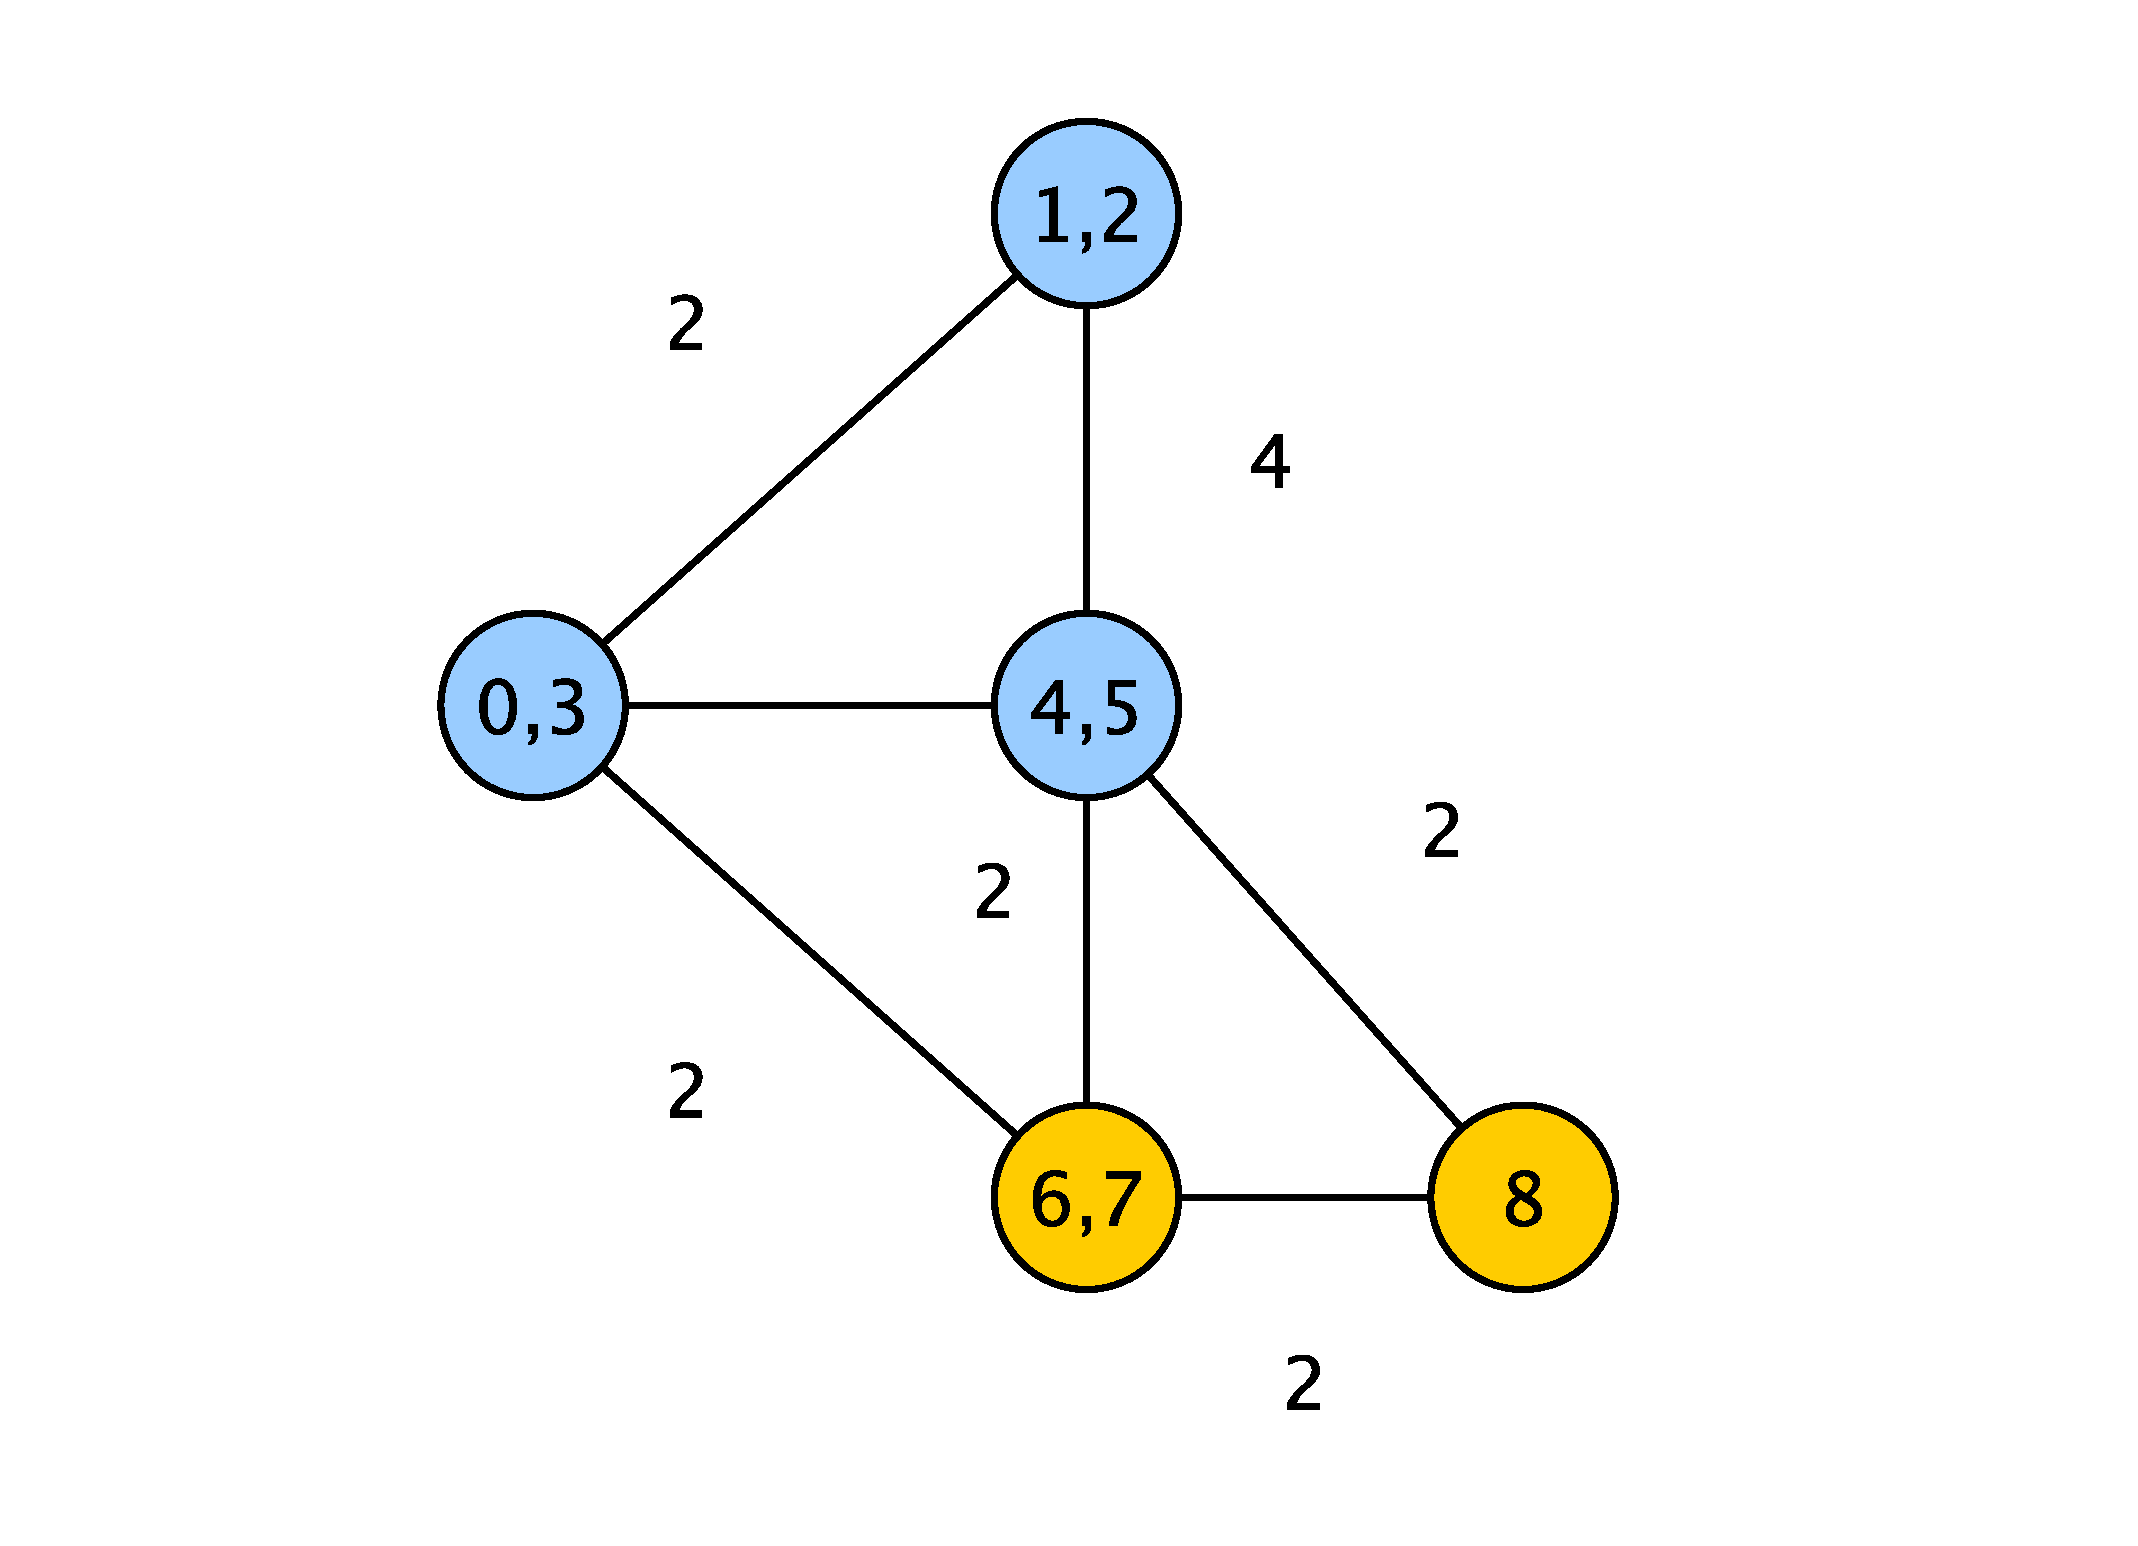
\includegraphics[scale=.15]{img/partition.eps}
    %\end{figure}
  %\end{center}

  %\column{.05\textwidth}{} 
  %\begin{center}
    %$\longrightarrow$  
  %\end{center}    
  
  %\column{.45\textwidth}{} 
  %\begin{center}
    %\begin{figure}[htbp]
      %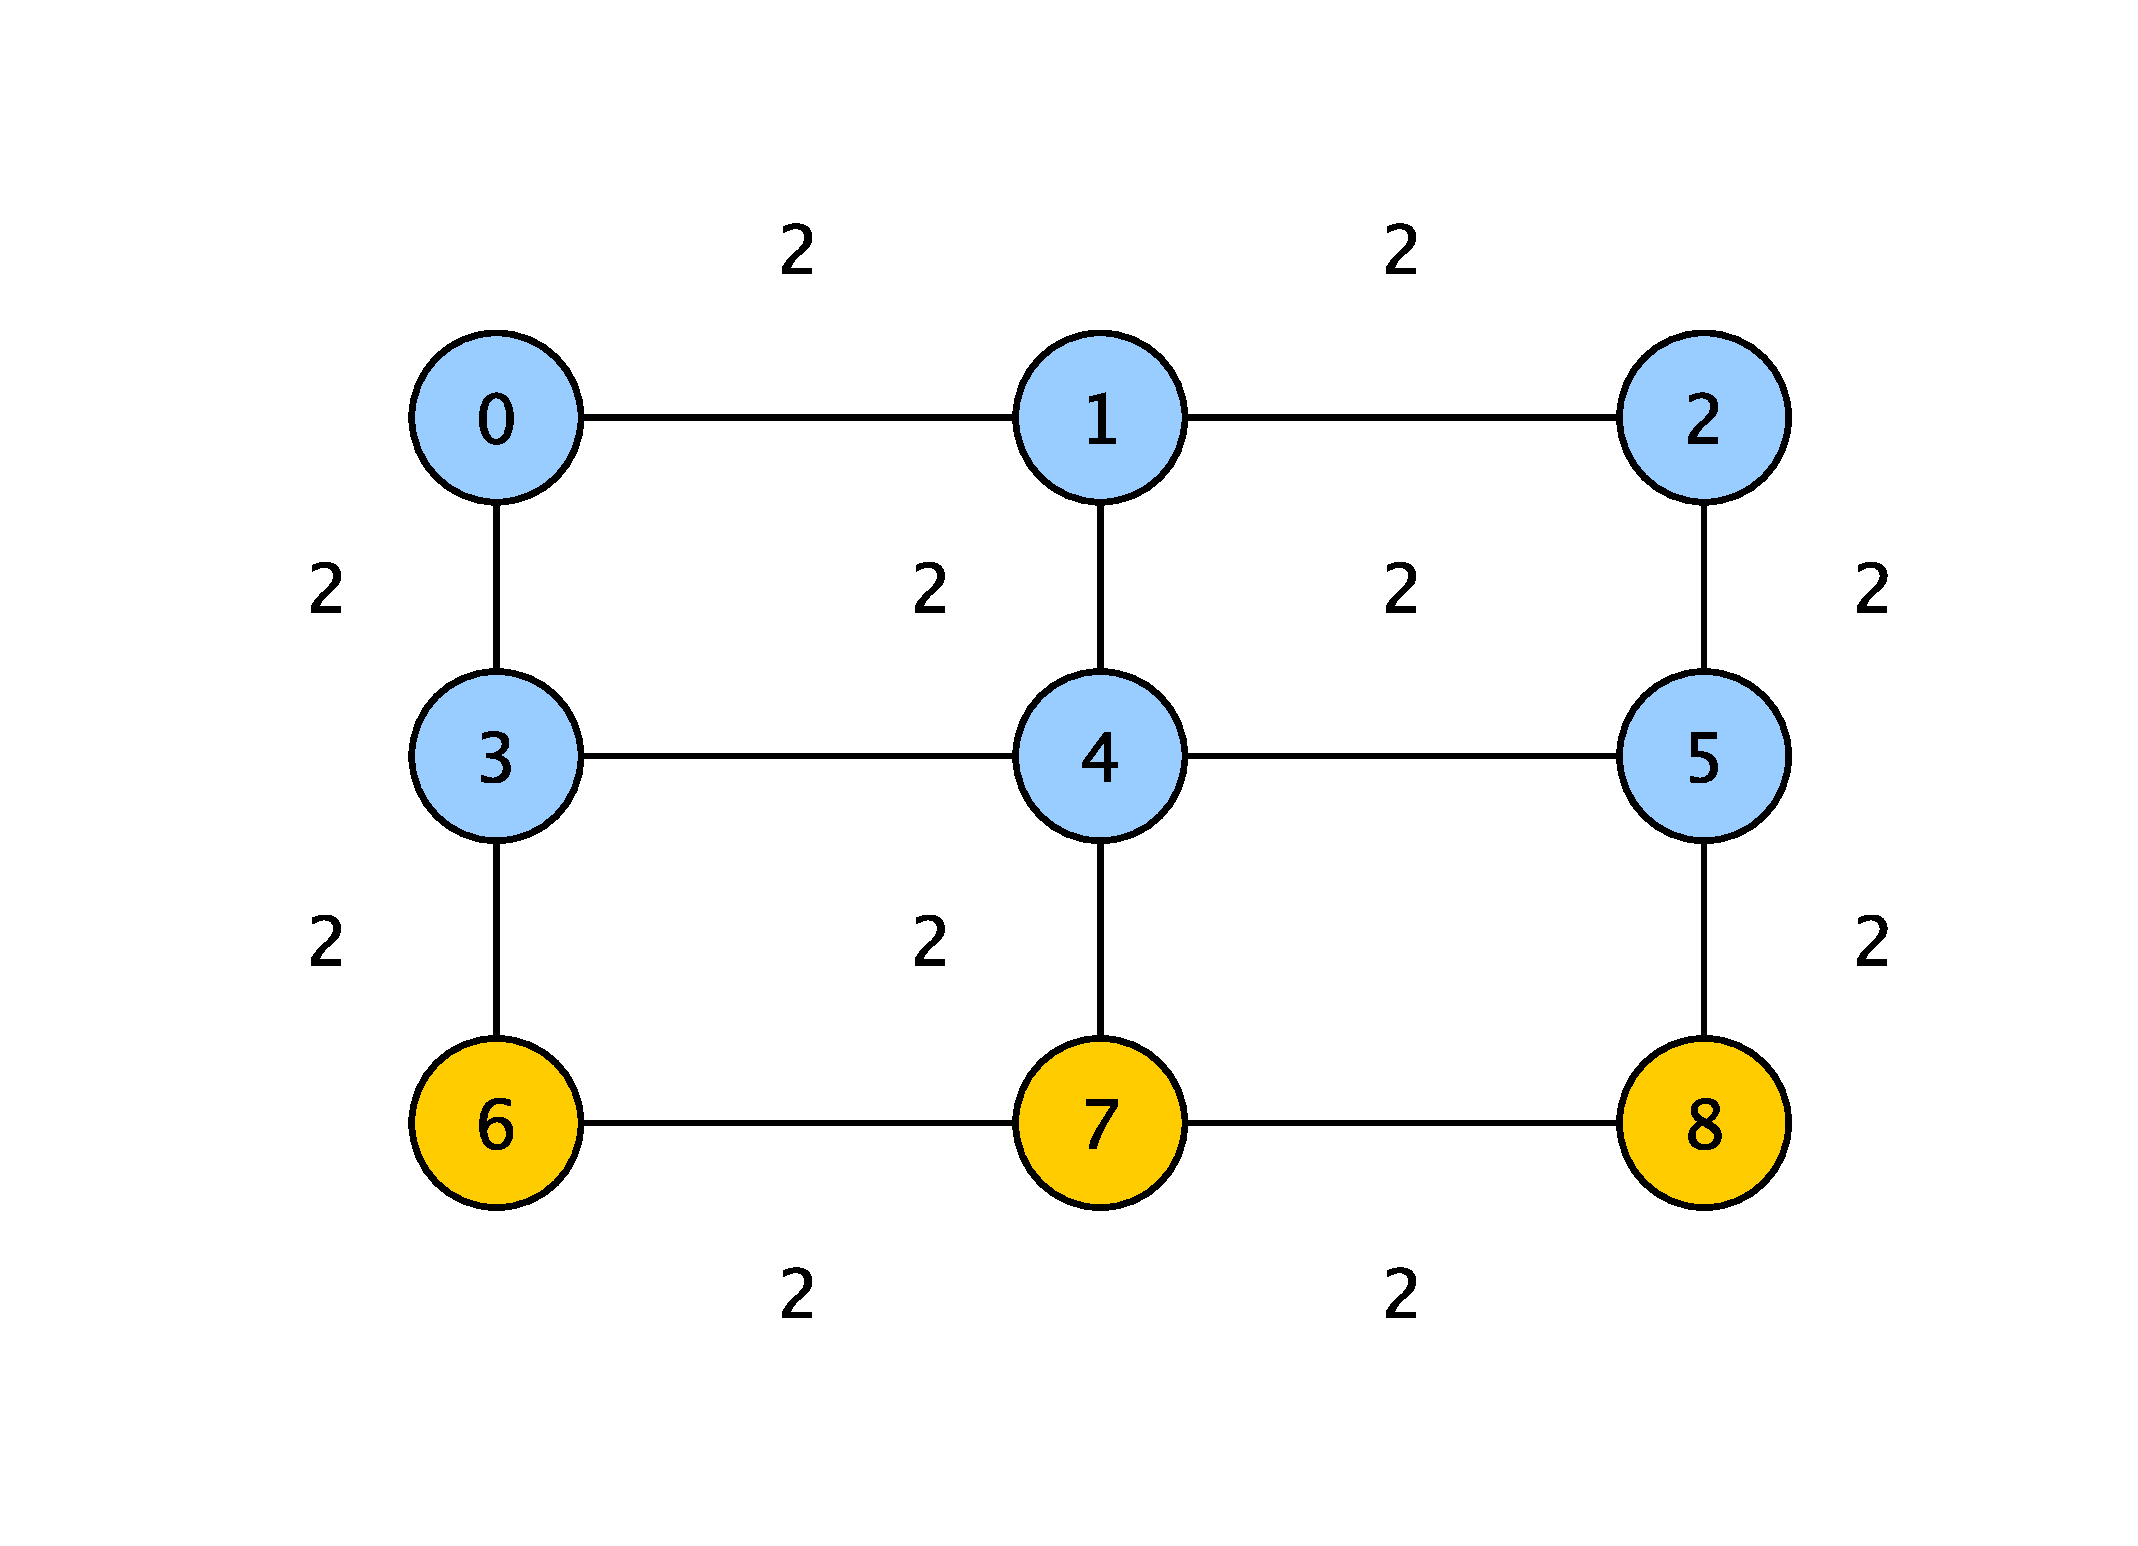
\includegraphics[scale=.15]{img/refinement.eps}
    %\end{figure}
  %\end{center}

%\end{columns}


%-----------------------------------------------------------------------------
% System characteristics
%-----------------------------------------------------------------------------

\section{System characteristics}

The measurements were performed in both Stampede's hosts and
coprocessors.
The hosts are comprised of dual Intel Xeon E5-2680, while the
coprocessors are the new Intel Xeon Phi with 61 cores. Their
characteristics are presented in the following tables.

\begin{table}[H]
\centering
\footnotesize
\begin{tabular}{| c | c |}\hline
Manufacturer & Intel\\ \hline
Model & Xeon E5-2680\\ \hline
$\mu$Arch & Sandy Bridge\\ \hline
Clock freq & 2.70 GHz\\ \hline
\#CPUs (sockets) & 2 \\ \hline
\#Cores/CPU & 8\\ \hline
\#Thread/Core & 1\\ \hline
L1 cache size/core & 32 KB\\ \hline
L2 cache size/core & 256 KB\\ \hline
L3 shared cache size/CPU & 20 MB\\ \hline
Main Memory/CPU & 16 GB\\ \hline
Vector width & 256 bits (AVX)\\ \hline
\end{tabular}
\caption{Intel Xeon E5-2680}
\end{table}

\begin{table}[H]
\centering
\footnotesize
\begin{tabular}{| c | c |}\hline
Manufacturer & Intel\\ \hline
Model & Xeon Phi SE10P\\ \hline
$\mu$Arch & Many Integrated Cores - MIC\\ \hline
Clock freq & 1.1 GHz\\ \hline
\#CPUs (sockets) & 1 \\ \hline
\#Cores/CPU & 61\\ \hline
\#Thread/Core & 4\\ \hline
L1 cache size/core & 32KB\\ \hline
L2 cache size/core & 512 KB\\ \hline
Main Memory/CPU & 8 GB\\ \hline
Vector width & 512 bits\\ \hline
\end{tabular}
\label{MIC}
\caption{Intel Xeon Phi}
\end{table}



%-----------------------------------------------------------------------------
% Xeon Phi
%-----------------------------------------------------------------------------

Apart from the characteristics showed in table~\ref{MIC}, there are
others that should be mentioned. Each core contains a in-order dual
pipeline which can issue two instructions from the same hardware thread
per clock cycle. However, the front-end of the pipeline does not issue
instructions from the same hardware thread in consecutive cycles.
%FIXME: Fazer um cite ao link que o andrew mandou por email
This means that the maximum issue rate is only attainable with at least
2 threads per core while the other threads have the purpose of hiding
pipeline stalls due to memory latency. %FIXME: Compor esta frase

The fact that the pipeline issue instructions in-order increases
memory related problems. %FIXME: Pode-se dar o exemplo do andrew

\begin{center}
\begin{figure}[htbp]
    \includegraphics[scale=.45]{img/phi_arch.jpg}
\end{figure}
\end{center}


%-----------------------------------------------------------------------------
% Metis %FIXME: Pôr isto mais acima?
%-----------------------------------------------------------------------------

\section{Metis}


%-----------------------------------------------------------------------------
% Mt-metis
%-----------------------------------------------------------------------------

\section{Mt-metis}

\begin{center}
\begin{figure}[htbp]
    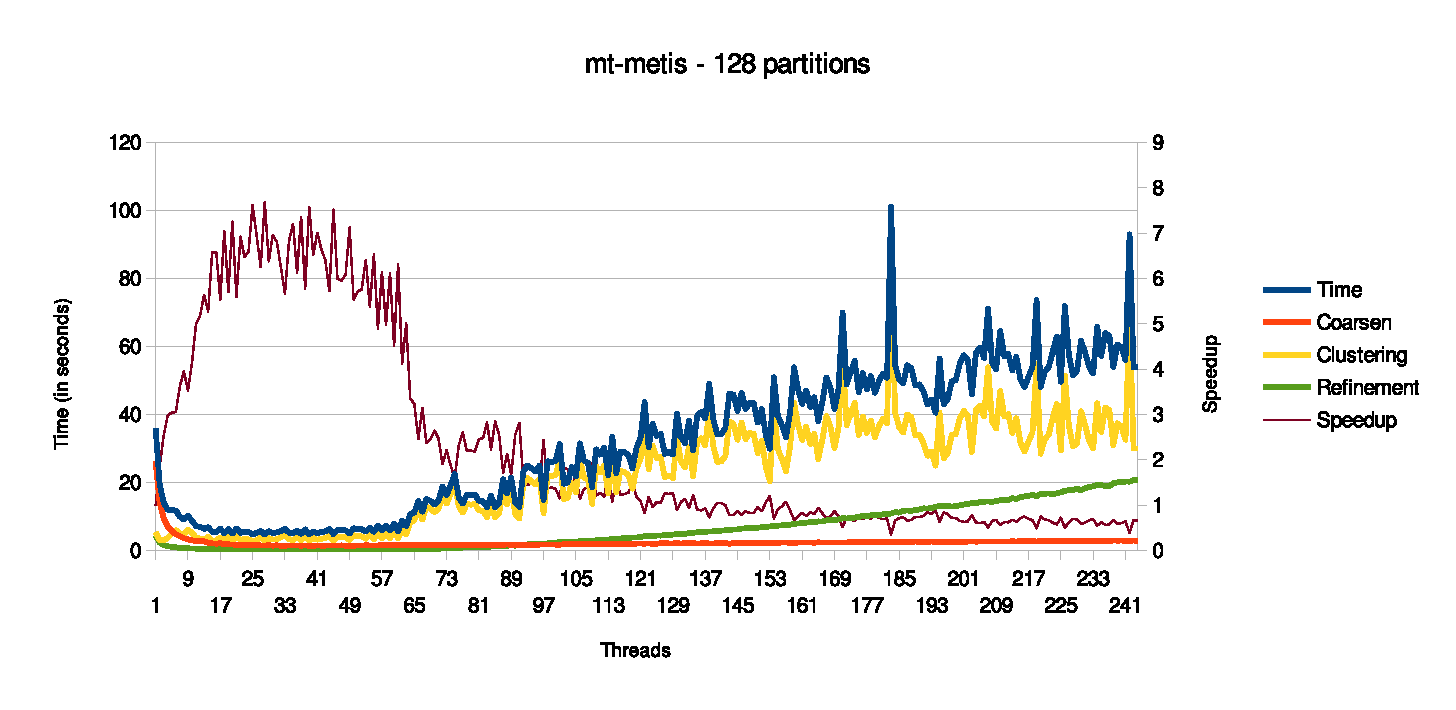
\includegraphics[scale=.40]{img/mtmetis128.eps}
    \caption{Mt-metis - 128 partitions}
\end{figure}
\end{center}


%-----------------------------------------------------------------------------
% GMetis and Galois Framework
%-----------------------------------------------------------------------------

\section{GMetis and the Galois Framework} %FIXME: Mudar o nome do titulo

\begin{center}
\begin{figure}[htbp]
    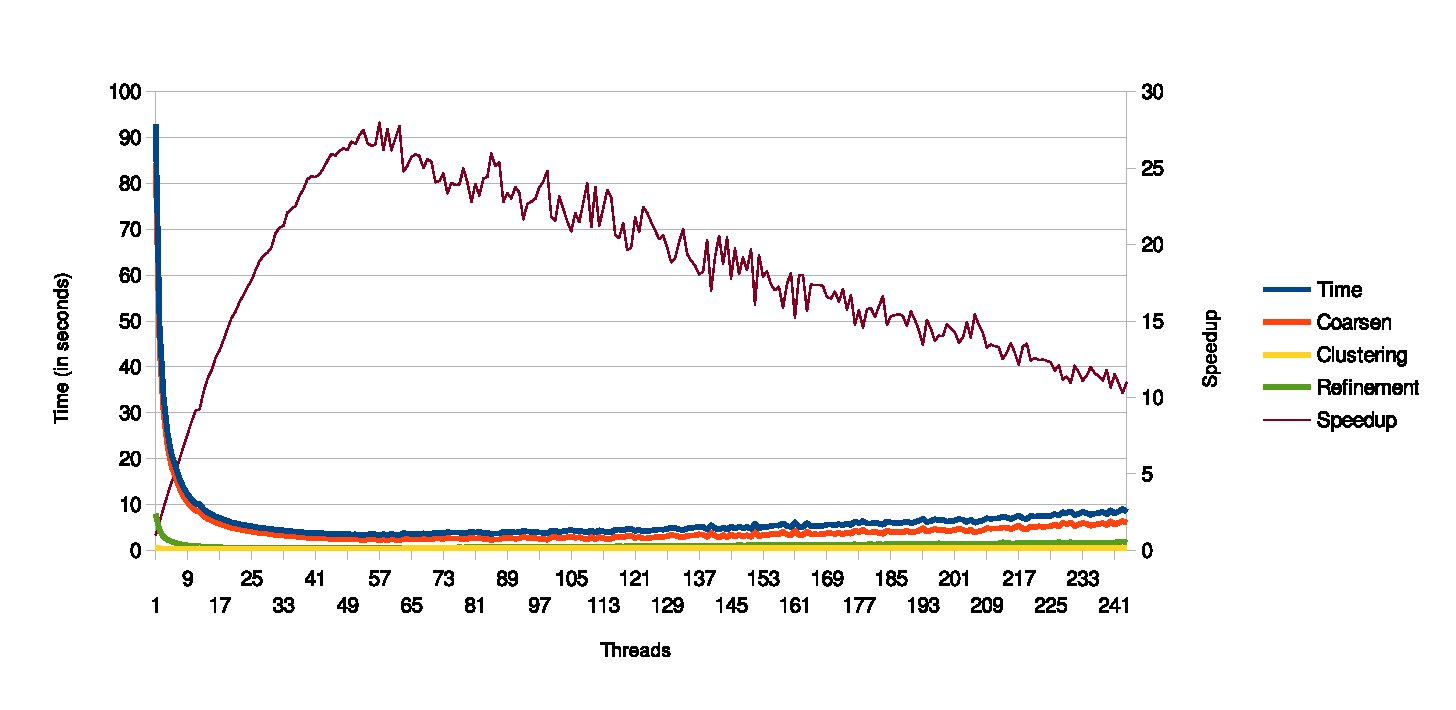
\includegraphics[scale=.40]{img/gmetis128.eps}
    \caption{GMetis - 128 partitions}
\end{figure}
\end{center}

This figure shows the scalability of gmetis on Xeon phi over the runtime
with on thread. This example is for 128 partition, but we did
measurements for different number of partitons, such as 16 and 1024. All
of them have a similar behaviour.

%-----------------------------------------------------------------------------
% Conclusion
%-----------------------------------------------------------------------------

\section{Conclusion}

Results showed that both \textit{Metis} and \textit{Mt-metis} have
better edgecut than \textit{Gmetis}. However, Gmetis's runtime is lower
for a high number of partitions.

%FIXME: Adicionar o número de partições em que o GMetis passa a ser mais
%rápido

Xeon Phi provides a theoretical performance of 2112 GFlop/sec for double
precision arithmetic and 1056 GFlops/sec for single precision
arithmetic. This values comprises the use of 60 cores since one core is
necessary to perform operating system operations.

%TODO: Falar sobre o facto do Sampede não ter o VTune com suporte para
%os MICs?


%-----------------------------------------------------------------------------
% Bibliography
%-----------------------------------------------------------------------------

%\bibliographystyle{plain}
%\bibliography{references}


\end{document}
